% ========================================
% Document Metadata
% ========================================
% Working number: #62
% DOI: 10.5281/zenodo.20091680
% Scope (Plan A): the input a as a frame-independent invariant with two
% representations; the modulus |a| as a geometric consequence; the factor
% 1/sqrt(2) as intrinsic to the conservation identity (velocity-level ratio).
% The exact correspondence between the derived velocity-level ratio and the
% canonical a-level placement (residual 2^{1/4}) is recorded as an open task.

\documentclass[%
 reprint, amsmath,amssymb, aps, prb, ]{revtex4-2}
% 基本パッケージ
\usepackage{graphicx}
\usepackage{bm}
% 量子力学記法
\usepackage{physics}
% ハイパーリンク
\usepackage[colorlinks=true,
            linkcolor=blue, filecolor=blue, urlcolor=blue, citecolor=blue]{hyperref}
% キャプション設定
\usepackage{caption}
\captionsetup[figure]{
    justification=raggedright, labelfont={bf}, name={Fig.}, labelsep=period }
\captionsetup[table]{
    labelfont={bf}, name={Table}, labelsep=period }
% 数式番号をセクションごとに
\numberwithin{equation}{section}
% タイポグラフィ調整
\tolerance=1000
\emergencystretch=1em
\hyphenpenalty=3000
\exhyphenpenalty=3000
\flushbottom
% マイクロタイポグラフィ
\usepackage[final]{microtype}
\usepackage{ragged2e}  % for \justifying command
% \midrule、\addlinespace、\bottomruleを使う
\usepackage{booktabs}
\usepackage{enumitem}
% Theorem environment
\usepackage{amsthm}
\newtheorem{theorem}{Theorem}[section]
% --- paragraph heading: run-in italic with extra top skip for block readability ---
\makeatletter
\renewcommand\paragraph{%
  \@startsection{paragraph}{4}{\z@}%
    {3mm \@plus 1ex \@minus .2ex}%   前 (block separator)
    {-1em}%                          後 (負値で run-in 維持)
    {\normalfont\normalsize\itshape}}
\makeatother
% Internal phase notation
\newcommand{\iphase}{\theta}  % internal geometric phase = ωt/2
\usepackage{tikz}
\usetikzlibrary{arrows.meta, calc, 3d, shadings, positioning, decorations.pathmorphing}
% --- Custom Macros ---
\newcommand{\omZB}{\omega_{\text{ZB}}}
\newcommand{\vZB}{v_{\text{ZB}}}
\newcommand{\gKE}{\gamma^{*}_{\text{KE}}}
\newcommand{\TPE}{\text{TPE}}
\newcommand{\gammaL}{\gamma_{L}}

\begin{document}

\title{The Bridge Equation $\gamma = 1 + a$ from First Principles:\\
Representation Duality of the Anomalous Moment and the Geometric\\
Origin of the Root-Mean-Square Factor in the 0-Sphere Model}

\author{Satoshi Hanamura}
\email{hana.tensor@gmail.com}
\date{June 13, 2026}

\begin{abstract}
The 0-Sphere model relates the anomalous magnetic moment $a$ of a spin-$1/2$ particle to the Lorentz factor of an internal Zitterbewegung oscillation through the bridge equation $\gamma = 1 + \lvert a\rvert$, with a velocity-determining variant $\gamma_v = 1 + \lvert a\rvert/\sqrt{2}$ carrying an explicit factor of $1/\sqrt{2}$.
This work supplies a first-principles foundation for both ends of that equation: the meaning of the input $a$ and the origin of the $1/\sqrt{2}$ factor in the transformation.
For the input, we argue that the anomalous moment is a single frame-independent invariant with two representations: externally, in a Penning trap, $a_e = T_c/T_a$ is a per-revolution phase slip accumulated over many cyclotron turns; internally, in the 0-Sphere model, $a_e = (L_0 - L)/L_0$ is the rotational Lorentz contraction of the internal orbital arc.
The factor $\gamma_L = 1 + a_e$ acts as a representation translator between a time ratio and a length ratio, in the same way a single Lorentz boost joins time dilation and length contraction.
We state the claim boundary with discipline: the field-independence of $a_e$ is \emph{consistent} with an internal-geometric representation but does not force it, since standard quantum electrodynamics is equally field-free.
For the transformation, we show that the $1/\sqrt{2}$ factor is not imported from an alternating-voltage analogy but is contained in the energy-conservation identity $\cos^4(\theta/2)+\sin^4(\theta/2)+\tfrac{1}{2}\sin^2\theta = 1$.
The momentum-carrying term $\gKE = \tfrac{1}{2}\sin^2\theta$ has a time-averaged-to-peak ratio whose square root is exactly $1/\sqrt{2}$; because the velocity is the square root of this term, identified through the relativistic decomposition $(mc^2/E)^2 + (pc/E)^2 = 1$, its cycle representative is necessarily the root-mean-square (RMS), not the peak.
We identify the geometric carrier as a pulsating-radius helix with $R(\theta)=(1/\sqrt{2})\lvert\sin\theta\rvert$, whose squared radius equals $\gKE$ exactly, vanishes on the kernels, and reaches maximum amplitude $1/\sqrt{2}$ at the midpoint, and we fix the internal winding number to unity through an SU(2) (720$^\circ$) amplitude versus U(1) (360$^\circ$) energy phase duality.
The result places the mass-determining peak factor and the velocity-determining RMS factor on a common footing as two readings of the same $\sin^2\theta$ partition, and establishes that the factor $1/\sqrt{2}$ is intrinsic to the identity rather than imported.
The placement of the factor is stated with the same discipline applied to the input: the ratio derived here is a velocity-level ratio, whereas the canonical form $\gamma_v = 1 + \lvert a\rvert/\sqrt{2}$ places the factor at the level of $a$; because the bridge relation is nonlinear, the two placements differ by a residual factor of $2^{1/4}$ at the velocity level, and their exact reconciliation is recorded as an open task rather than asserted.
An appendix records the line-integral genealogy of the construction and the inverse-direction use of geometry across the model.
\end{abstract}

\maketitle

\section{Introduction}
\label{sec:intro}

The 0-Sphere model describes a free electron as a thermodynamically closed system in which energy oscillates between two localized kernels, A and B, mediated by an internal photon sphere~\cite{hanamura01}. The total rest energy is partitioned according to a single internal phase $\theta=\omega t$ through the conservation identity
\begin{equation}
E_0 = E_0\!\left[\cos^4\!\left(\frac{\theta}{2}\right) + \sin^4\!\left(\frac{\theta}{2}\right) + \frac{1}{2}\sin^2\theta\right],
\label{eq:identity}
\end{equation}
where the first two terms are the thermal potential energies (TPE) of the kernels and the third, $\gKE=\tfrac{1}{2}\sin^2\theta$, is the kinetic energy of the photon sphere~\cite{hanamura01}. A central quantitative result of the model is the bridge equation relating the experimentally measured anomalous magnetic moment $a$ to the internal Zitterbewegung velocity. In its mass-determining form it reads $\gamma = 1 + \lvert a\rvert$, and in its velocity-determining form $\gamma_v = 1 + \lvert a\rvert/\sqrt{2}$, the latter carrying an explicit factor of $1/\sqrt{2}$~\cite{hanamura10,hanamura61}. Two distinct questions attach to this single equation, and this paper addresses both. The first concerns the \emph{input}: what kind of quantity is the anomalous moment $a$, that it should enter a relation between an externally measured magnetic anomaly and an internal kinematic velocity? The second concerns the \emph{transformation}: why does the velocity-determining form carry the specific factor $1/\sqrt{2}$? We treat the input in Sec.~\ref{sec:duality-rep} as a representation duality of a single frame-independent invariant, and the transformation in Secs.~\ref{sec:momentum}--\ref{sec:winding} as a structural consequence of the conservation identity.

In an earlier work~\cite{hanamura10} the velocity relation was written as
\begin{equation}
\sqrt{1-\frac{v^2}{c^2}} = \frac{1}{1+\frac{1}{\sqrt{2}}\,a_e},
\label{eq:bridge}
\end{equation}
yielding $\vZB \approx 0.04047c$. The factor $1/\sqrt{2}$ appearing in the denominator was introduced there by explicit analogy: it was argued that, just as an alternating voltage is characterized by its RMS value rather than its peak, the fluctuating Lorentz contraction driven by the harmonic oscillator should be represented by the RMS of $a_e$ rather than its peak~\cite{hanamura10}. The same reference noted that the peak value of $a_e$, obtained by omitting $1/\sqrt{2}$, gives the instantaneous maximum velocity $v_{\max}\approx 0.0481c$, and characterized the value obtained from the RMS of $a_e$ as the cycle-averaged velocity; note that throughout, the historical placement of the factor is on $a_e$, a point to which we return in Sec.~\ref{sec:momentum}.

This heuristic has remained an interpretive placeholder. The original derivation explicitly deferred its justification, stating that further observation would confirm the choice~\cite{hanamura10}. The purpose of the present work is to supply that justification from first principles. We show that the factor $1/\sqrt{2}$ is not imported from an external analogy but is already contained in the structure of the identity~\eqref{eq:identity}. Specifically, the momentum-carrying term $\gKE=\tfrac{1}{2}\sin^2\theta$ has a definite ratio between its time average and its peak, and the square root of that ratio is exactly $1/\sqrt{2}$. Since the internal velocity is proportional to the square root of the momentum term, its representative value over a cycle is necessarily the RMS.

We then identify the geometric object that carries this term. Building on the helical-trajectory description of the photon sphere~\cite{hanamura51} and the thermal-geodesic framework~\cite{hanamura24}, we replace the constant-radius helix with a pulsating-radius helix whose squared radius equals the momentum term $\gKE$ exactly. This helix vanishes on the kernels---recovering the stationary points where the photon-sphere momentum is zero~\cite{hanamura07}---and reaches a maximum amplitude of $1/\sqrt{2}$ at the midpoint between them. The coincidence of this maximum amplitude with the RMS factor is not accidental: both are the square root of the same ratio.

Finally, we clarify which internal winding the velocity description must use. The identity~\eqref{eq:identity} contains two phase scales: the kernel amplitudes evolve in $\theta/2$ (720$^\circ$, SU(2)), while the kinetic energy evolves in $\theta$ (360$^\circ$, U(1))~\cite{hanamura01,hanamura19}. Because the velocity is a property of the kinetic term, the relevant winding number is unity. With this choice the helical projection reproduces $1/\sqrt{2}$ exactly. The result unifies three apparently distinct routes to the same factor and places the mass-determining and velocity-determining structures of the model on a common footing. One distinction is maintained carefully throughout: what the identity yields is a velocity-level ratio (cycle-representative velocity to peak velocity), whereas the canonical form $\gamma_v = 1+\lvert a\rvert/\sqrt{2}$ places the factor at the level of $a$; because the bridge relation is nonlinear, these placements are not equivalent, and their exact correspondence is recorded as an open task in Sec.~\ref{sec:momentum} rather than asserted.

The paper is organized as follows. Section~\ref{sec:duality-rep} treats the input side, presenting the anomalous moment as a single frame-independent invariant with an external (time-ratio) and an internal (length-ratio) representation, and establishes the claim boundary with discipline. Section~\ref{sec:momentum} establishes the time-average-to-peak structure of the momentum term and derives $1/\sqrt{2}$ from the identity alone, grounded in the relativistic energy--momentum decomposition. Section~\ref{sec:helix} constructs the pulsating-radius helix, shows $R^2=\gKE$, and recovers the stationary points. Section~\ref{sec:winding} develops the SU(2)/U(1) phase duality and fixes the winding number. Section~\ref{sec:discussion} relates the result to the mass-versus-velocity asymmetry and to prior work. Appendix~\ref{app:genealogy} records the line-integral genealogy and the inverse-direction use of geometry across the model. Appendix~\ref{app:setaside} records two internal ratios that were examined and set aside as lacking a confirmed connection to observables.

\section{The Anomalous Moment as a Frame-Independent Invariant}
\label{sec:duality-rep}

Before analyzing the transformation factor, we address the input. The bridge equation~\eqref{eq:bridge} relates a measured magnetic anomaly to an internal kinematic velocity, and it is natural to ask what single quantity could legitimately stand on both sides. We argue that the anomalous magnetic moment is one invariant carried in two representations, and that $\gamma_L = 1 + a_e$ is the translator between them.

\paragraph{The external representation: a per-revolution phase slip.}
In a Penning trap the electron anomalous moment is measured as the ratio of two frequencies, the anomaly frequency and the cyclotron frequency~\cite{codata2022}, or equivalently as a ratio of two characteristic times,
\begin{equation}
a_e = \frac{T_c}{T_a},
\label{eq:ae-external}
\end{equation}
where $T_c$ is the cyclotron period and $T_a$ the anomaly period. Physically this is a per-revolution phase slip: the spin precesses slightly faster than the cyclotron motion, and $a_e$ is the fractional advance accumulated per turn. It is an externally accumulated, observationally defined time ratio.

\paragraph{The internal representation: a rotational length contraction.}
In the 0-Sphere model the same number appears as a length ratio,
\begin{equation}
a_e = \frac{L_0 - L}{L_0},
\label{eq:ae-internal}
\end{equation}
where $L_0$ is the rest arc length of the internal orbital motion and $L$ its rotationally Lorentz-contracted value~\cite{hanamura10,hanamura47}. Here $a_e$ measures the fractional contraction of the internal arc traversed by the photon sphere. It is an internally defined geometric length ratio.

\paragraph{One invariant, two projections.}
Equations~\eqref{eq:ae-external} and~\eqref{eq:ae-internal} assign the same numerical value to $a_e$ through two operationally distinct procedures, one external and temporal, the other internal and spatial. The relation
\begin{equation}
\gamma_L = 1 + a_e
\label{eq:gammaL-translator}
\end{equation}
acts as a representation translator between them, in precise analogy with special relativity, where a single Lorentz boost simultaneously dilates time and contracts length and a single $\gamma$ joins the two. The anomalous moment is, in this reading, a frame-independent invariant: a time ratio when registered externally, a length ratio when registered internally, the two joined by Eq.~\eqref{eq:gammaL-translator}.

\paragraph{The length-ratio representation is non-negative: origin of the modulus.}
The internal representation~\eqref{eq:ae-internal} fixes the sign character of the quantity that enters the bridge equation, and this resolves a question that the external representation alone leaves open. Externally, the measured anomalous moment carries a sign---it is positive for the proton and the electron but negative for the neutron and for certain other particles---and one may ask which sign the bridge equation $\gamma = 1 + \lvert a\rvert$ should respect. The internal representation answers this geometrically. The internal arc contraction is a rotational Lorentz contraction: the orbital arc of rest length $L_0 = 2\pi r$, traversed by the photon sphere at the internal velocity $\vZB$, contracts to $L = L_0/\gammaL$ with $\gammaL = (1 - \vZB^2/c^2)^{-1/2}$, so that the fractional deficit is $a_e \approx (L_0 - L)/L_0$. The contraction factor depends on the internal speed only through $\vZB^2/c^2$, and the square enters because length contraction is governed by the squared speed, not the velocity vector. Consequently the arc deficit is the same whether the internal circulation is clockwise or counterclockwise: reversing the sense of rotation reverses the direction of the velocity vector but leaves $\vZB^2$, and therefore the contraction, unchanged. The two senses of rotation are illustrated in Fig.~\ref{fig:arc_modulus}. The length ratio $(L_0 - L)/L_0$ is thus intrinsically non-negative, a contraction deficit that cannot be made negative by any choice of circulation sense. In the internal representation, then, the quantity identified with the anomalous moment is the magnitude of the contraction, and the modulus form $\gamma = 1 + \lvert a\rvert$ is the geometric consequence of this fact rather than a convention imposed by hand. When an external measurement reports a negative anomalous moment, the 0-Sphere internal representation reads that value as the same non-negative arc-contraction deficit, the external sign being a property of the magnetic-response orientation rather than of the internal length ratio. We hold this to the same claim boundary adopted throughout the section: the modulus is a structural property of the length-ratio representation, and we do not assert thereby that the internal representation is the privileged or sole account of the sign of the magnetic response.

\begin{figure*}[t!]
\centering
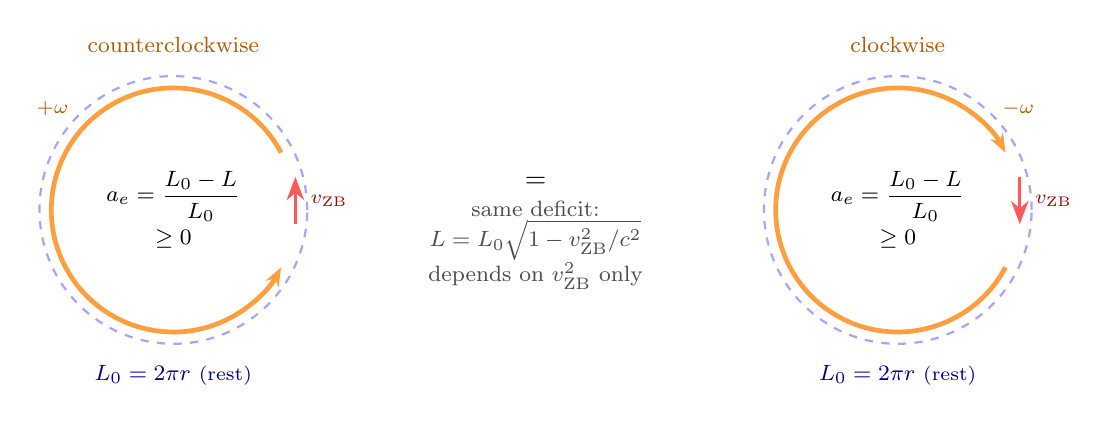
\begin{tikzpicture}[>=Stealth, font=\small]
% ===== Left panel: counterclockwise circulation =====
\begin{scope}[shift={(-4.6,0)}]
  % uncontracted reference (rest arc)
  \draw[blue!35, thick, dashed] (0,0) circle (1.7);
  % contracted arc (slightly inset, counterclockwise arrow)
  \draw[orange!75, line width=1.7pt, -{Stealth[length=2.4mm]}]
    (28:1.55) arc (28:332:1.55);
  % rotation-sense label
  \node[font=\footnotesize, orange!70!black] at (90:2.1) {counterclockwise};
  \node[font=\scriptsize, orange!70!black] at (140:2.0) {$+\omega$};
  % rest-length label on dashed circle
  \node[font=\footnotesize, blue!55!black] at (270:2.1) {$L_0 = 2\pi r$ \scriptsize(rest)};
  % velocity vector at right, pointing up (CCW tangent)
  \draw[->, red!65, very thick] (1.55,-0.18) -- (1.55,0.42);
  \node[font=\scriptsize, red!65!black, right] at (1.62,0.12) {$\vZB$};
  % arc deficit callout
  \node[font=\footnotesize, align=center] at (0,0)
    {$a_e=\dfrac{L_0-L}{L_0}$\\[2pt]$\ge 0$};
\end{scope}
% ===== Right panel: clockwise circulation =====
\begin{scope}[shift={(4.6,0)}]
  \draw[blue!35, thick, dashed] (0,0) circle (1.7);
  % contracted arc, clockwise arrow (reverse the arc direction)
  \draw[orange!75, line width=1.7pt, -{Stealth[length=2.4mm]}]
    (332:1.55) arc (332:28:1.55);
  \node[font=\footnotesize, orange!70!black] at (90:2.1) {clockwise};
  \node[font=\scriptsize, orange!70!black] at (40:2.0) {$-\omega$};
  \node[font=\footnotesize, blue!55!black] at (270:2.1) {$L_0 = 2\pi r$ \scriptsize(rest)};
  % velocity vector at right, pointing down (CW tangent)
  \draw[->, red!65, very thick] (1.55,0.42) -- (1.55,-0.18);
  \node[font=\scriptsize, red!65!black, right] at (1.62,0.12) {$\vZB$};
  \node[font=\footnotesize, align=center] at (0,0)
    {$a_e=\dfrac{L_0-L}{L_0}$\\[2pt]$\ge 0$};
\end{scope}
% ===== Center: equality of the two deficits =====
\node[font=\normalsize] at (0,0.35) {$=$};
\node[font=\footnotesize, align=center, gray!60!black] at (0,-0.45)
  {same deficit:\\ $L=L_0\sqrt{1-\vZB^2/c^2}$\\ depends on $\vZB^2$ only};
\end{tikzpicture}
\caption{\textbf{Rotation-sense independence of the internal arc contraction}}
\label{fig:arc_modulus}
\vspace{0.4em}
\begin{minipage}{0.95\textwidth}
\justifying\small
The internal orbital arc of rest circumference $L_0 = 2\pi r$ (dashed blue) contracts to $L = L_0\sqrt{1-\vZB^2/c^2}$ (solid orange) when traversed by the photon sphere at the internal velocity $\vZB$. Left: counterclockwise circulation ($+\omega$); right: clockwise circulation ($-\omega$). Reversing the sense of rotation reverses the velocity vector $\vZB$ but leaves $\vZB^2$, and therefore the contraction factor $\gammaL = (1-\vZB^2/c^2)^{-1/2}$, unchanged. The fractional arc deficit $a_e = (L_0-L)/L_0$ is identical in the two cases and is intrinsically non-negative. This is the geometric origin of the modulus in the bridge equation $\gamma = 1 + \lvert a\rvert$: the quantity identified with the anomalous moment in the internal representation is a length-contraction deficit, which carries no sign.
\end{minipage}
\end{figure*}

\paragraph{Three-scale separation.}
The two readings live at widely separated scales. Three characteristic periods enter: the external cyclotron period $T_c \sim 10^{-12}$~s, the external anomaly period $T_a \sim 10^{-9}$~s, and the internal Zitterbewegung period $T_{ZB} \sim 10^{-19}$~s, with the nesting $T_c/T_{ZB} \approx 3.4\times10^{7}$. The two external periods depend on the trap magnetic field $B$; the internal period does not. Yet $a_e$ itself is $B$-independent in both layers. The anomalous moment is thus the unique $B$-independent invariant standing at the intersection of a field-dependent observational layer and a field-independent internal-geometric layer.

\paragraph{The claim boundary, stated with discipline.}
It is tempting to argue that, because $a_e$ is field-independent, its origin must be the field-independent internal geometry. We do not make this claim, and the discipline matters. Standard quantum electrodynamics computes $a_e$ as a field-free vertex correction; field-independence is therefore equally a property of the standard account and cannot by itself select between descriptions. The exact and defensible statement is weaker and is the one we adopt throughout: the internal-kinematic representation $\gamma_L = 1 + a_e$ is \emph{consistent} with the field-independent character of $a_e$, and is not in conflict with it. This modest-articulation posture matches the discipline applied elsewhere in the model where a numerical correspondence is established before its mechanism is known~\cite{hanamura28}. What the present section establishes is a representation duality of the input, not a proof that the internal representation is privileged.

\paragraph{The apparent loop.}
One feature of the external representation deserves comment because it connects to the line-integral structure used later. The Penning-trap orbital integral is naturally read as a closed loop, yet in the 0-Sphere model a genuinely closed internal trajectory does not exist; the photon-sphere process is open, $A \to B \to A'$ with $A' \neq A$. The external closed loop is therefore an \emph{apparent loop observable}: a closed quantity assembled from open-path residuals under the closure constraint imposed by interference-style measurement. This composition---a closed loop built as the difference of open paths under an observational constraint---is the line-integral reading developed in the genealogy of Appendix~\ref{app:genealogy}. We flag it here only to mark that the external time-ratio representation and the internal length-ratio representation are both line-integral quantities, differing in whether the integration path is read as closed (external, constrained) or open (internal, fundamental).

\section{The Momentum Term and the Origin of \texorpdfstring{$1/\sqrt{2}$}{1/sqrt2}}
\label{sec:momentum}

The starting point is the relativistic interpretation of the three terms in Eq.~\eqref{eq:identity}. The model reads the identity as a partition of the dispersion relation $E^2=(mc^2)^2+(pc)^2$ into a mass sector and a momentum sector~\cite{hanamura07}. Using the elementary identity
\begin{equation}
\cos^4\!\left(\frac{\theta}{2}\right) + \sin^4\!\left(\frac{\theta}{2}\right) = 1 - \frac{1}{2}\sin^2\theta,
\label{eq:tpe-reduce}
\end{equation}
the conservation law~\eqref{eq:identity} separates cleanly into the mass term $1-\tfrac{1}{2}\sin^2\theta$ and the momentum term
\begin{equation}
\gKE = \frac{1}{2}\sin^2\theta,
\label{eq:momentum-term}
\end{equation}
with the two summing to unity at every phase. The velocity follows from the dispersion relation as the square root of the momentum fraction,
\begin{equation}
\frac{v}{c} = \frac{pc}{E} = \sqrt{\gKE} = \frac{1}{\sqrt{2}}\,\lvert\sin\theta\rvert.
\label{eq:velocity-sqrt}
\end{equation}
This is the structural fact on which everything else rests: \emph{the velocity is the square root of a quantity that varies as $\sin^2\theta$}.

\paragraph{Time average versus peak.}
A quantity proportional to $\sin^2\theta$ does not have a single value over a cycle; it ranges between zero and its peak. The momentum term reaches its maximum at the midpoint $\theta=\pi/2$,
\begin{equation}
\max_\theta \gKE = \frac{1}{2},
\label{eq:peak}
\end{equation}
while its time average over a full cycle is
\begin{equation}
\langle \gKE \rangle = \frac{1}{2\pi}\int_0^{2\pi}\frac{1}{2}\sin^2\theta\,d\theta = \frac{1}{4}.
\label{eq:average}
\end{equation}
The representative velocity is obtained by taking the square root of the momentum term, so the cycle-representative velocity is governed by the square root of the average-to-peak ratio,
\begin{equation}
\sqrt{\frac{\langle \gKE \rangle}{\max_\theta \gKE}} = \sqrt{\frac{1/4}{1/2}} = \frac{1}{\sqrt{2}}.
\label{eq:rms-origin}
\end{equation}

Equation~\eqref{eq:rms-origin} is the central result of this section. The same number $1/\sqrt{2}$ that appears in the bridge relation~\eqref{eq:bridge} is here obtained as the square root of the ratio between the time-averaged and peak values of the momentum term; the factor is therefore not an external RMS correction imported by analogy but a quantity intrinsic to the identity~\eqref{eq:identity}. What this establishes, stated precisely, is a velocity-level ratio: the cycle-representative velocity stands to the peak velocity in the ratio $1/\sqrt{2}$. How this ratio corresponds to the placement of the factor in the canonical form $\gamma_v = 1 + \lvert a\rvert/\sqrt{2}$, where the factor multiplies $a$ rather than the velocity, is a distinct question, and we address it explicitly below.

\paragraph{The placement of the factor: an open correspondence.}
The bridge relation is nonlinear, so a ratio cannot be transported unchanged between the $a$-slot and the velocity-slot. For the electron, where $a_e$ is small, the relation gives $v \approx c\sqrt{2a}$ at leading order; replacing $a \to a/\sqrt{2}$ therefore scales the velocity by $2^{-1/4} \approx 0.841$, whereas a velocity-level factor of $1/\sqrt{2} \approx 0.707$ scales it directly. Numerically, the canonical placement $\gamma_v = 1+\lvert a\rvert/\sqrt{2}$ yields $\vZB \approx 0.0405c$~\cite{hanamura10}, while the velocity-level reading of the same profile, $v_{\max}/\sqrt{2}$, yields $\approx 0.0340c$; the two differ by the residual factor $2^{1/4} \approx 1.19$. The present derivation establishes that the identity contains the number $1/\sqrt{2}$ as the representative-to-peak ratio of the velocity; it does not by itself establish that the factor belongs at the level of $a$. We therefore hold the claim to the boundary it supports: the factor is identity-intrinsic, the asymmetry between the peak (mass) and cycle-representative (velocity) readings is structural, and the exact correspondence between the derived velocity-level ratio and the canonical $a$-level placement --- equivalently, the origin of the residual $2^{1/4}$ --- is recorded as an open task. A candidate route is noted without commitment: the pulsating radius of Sec.~\ref{sec:helix} is linear in $\lvert\sin\theta\rvert$, so a contraction deficit proportional to the transverse amplitude would carry exactly the profile whose cycle representative reproduces the $a$-level placement; whether such a proportionality can be established from the rotational-contraction geometry is part of the open task.

\paragraph{Why the square root forces the RMS.}
The distinction between this argument and the original AC analogy is worth stating precisely. The AC analogy asserts a correspondence; the present argument derives a value. Because the observable velocity is $\sqrt{\gKE}$ rather than $\gKE$ itself, a quantity that is quadratic in $\sin\theta$ at the energy level becomes linear in $\lvert\sin\theta\rvert$ at the velocity level. The conservation identity~\eqref{eq:identity} is the normalized form of the relativistic energy--momentum relation: the mass term $\cos^4(\theta/2)+\sin^4(\theta/2)=1-\gKE$ plays the role of $(mc^2/E)^2$ and the momentum term $\gKE$ that of $(pc/E)^2$, the two summing to unity at every phase exactly as $(mc^2/E)^2+(pc/E)^2=1$. The velocity enters only as the derived quantity $v/c=pc/E=\sqrt{\gKE}$; the quantities that are linearly conserved and partitioned along the cycle are the energy terms, not the velocity. The cycle representative must therefore be taken at the level of the conserved energy quantity, with the velocity following as its square root rather than the reverse. The natural cycle representative of a quadratic energy quantity is its mean; the corresponding velocity is the square root of that mean, normalized to the peak---which is exactly the RMS. A simple-average treatment of $\lvert\sin\theta\rvert$ would instead give $2/\pi\approx0.637$, and a naive factor of $1/2$ would give $0.5$; neither equals the identity-intrinsic value $1/\sqrt{2}\approx0.707$. The identity selects the RMS uniquely because the velocity is a square-root quantity built on a $\sin^2\theta$ momentum term.

\section{The Pulsating-Radius Helix}
\label{sec:helix}

The momentum term~\eqref{eq:momentum-term} admits a direct geometric realization. We seek a helical trajectory for the internal photon sphere whose squared radius equals the momentum content at every phase. Setting the helix radius to
\begin{equation}
R(\theta) = \frac{1}{\sqrt{2}}\,\lvert\sin\theta\rvert,
\label{eq:radius}
\end{equation}
the squared radius reproduces the momentum term exactly,
\begin{equation}
R^2(\theta) = \frac{1}{2}\sin^2\theta = \gKE .
\label{eq:R2}
\end{equation}
The radius is therefore not a free parameter but the geometric image of the kinetic energy: the transverse extent of the internal motion at each phase is fixed by the momentum fraction carried at that phase.

\paragraph{Why the radius must vary.}
The constant-radius helix used previously~\cite{hanamura51} cannot represent this structure, because the driving force of the internal oscillation is itself phase-dependent. The thermal gradient between the kernels is~\cite{hanamura01}
\begin{equation}
\nabla(T_{e2}-T_{e1}) = E_0\sin\theta,
\label{eq:gradient}
\end{equation}
which is the time derivative of the quartic kernel energies and is manifestly not constant. A force that varies as $\sin\theta$ cannot drive a motion of constant transverse amplitude; the amplitude must itself vary with phase. Equation~\eqref{eq:radius} is the variation consistent with $R^2$ equal to the momentum term.

\paragraph{Recovery of the stationary points.}
The pulsating radius vanishes on the kernels,
\begin{equation}
R(0)=R(\pi)=0,
\label{eq:kernel-vanish}
\end{equation}
and reaches its maximum at the midpoint,
\begin{equation}
R\!\left(\frac{\pi}{2}\right)=\frac{1}{\sqrt{2}} .
\label{eq:midpoint-max}
\end{equation}
At the kernels the transverse motion disappears and the entire energy resides in the mass term, recovering the stationary points where the photon-sphere momentum vanishes, $p_{\gamma^{*}}=0$~\cite{hanamura07}. This is the geometric counterpart of the relativistic statement that the velocity~\eqref{eq:velocity-sqrt} is zero at $\theta=n\pi$ and maximal at the midpoint. The constant-radius description does not reproduce this behaviour, since its transverse motion never vanishes; the pulsating-radius helix is the description faithful to the two-kernel architecture.

\paragraph{Coincidence of the maximum amplitude with the RMS factor.}
The maximum radius~\eqref{eq:midpoint-max} equals $1/\sqrt{2}$, numerically identical to the factor derived in Eq.~\eqref{eq:rms-origin}. This is not a coincidence. Both quantities are square roots of the momentum term: the maximum radius is $\sqrt{\max_\theta\gKE}=\sqrt{1/2}=1/\sqrt{2}$, while the RMS factor is $\sqrt{\langle\gKE\rangle/\max_\theta\gKE}$. The shared appearance of $1/\sqrt{2}$ reflects the common origin in $\gKE=\tfrac{1}{2}\sin^2\theta$. The helix is thus not merely consistent with the result of Sec.~\ref{sec:momentum}; it is the same statement expressed geometrically.

\section{SU(2) Amplitude and U(1) Energy: Fixing the Winding}
\label{sec:winding}

The construction of Sec.~\ref{sec:helix} requires a choice: how many internal rotations the photon sphere completes per traversal between kernels. We show that this choice is fixed by the phase structure of the identity~\eqref{eq:identity} rather than being free.

\paragraph{Two phase scales in one identity.}
The identity carries a single internal phase $\theta=\omega t$, but its terms register that phase at two different scales. The kernel amplitudes are built on $\cos(\theta/2)$ and $\sin(\theta/2)$, which have period $4\pi$ in $\theta$ (720$^\circ$); these are the spinorial, SU(2) objects. Yet their fourth powers, the thermal energies $\cos^4(\theta/2)$ and $\sin^4(\theta/2)$, have period $2\pi$ (360$^\circ$), because raising to the fourth power symmetrizes the sign change under $\theta\to\theta+2\pi$. The kinetic term $\tfrac{1}{2}\sin^2\theta$ likewise registers at the energy scale of $2\pi$. The single internal phase therefore presents a $720^\circ$ structure at the amplitude level and a $360^\circ$ structure at the energy level. This is the precise sense in which the model treats SU(2) and U(1) on a common footing~\cite{hanamura19}: they are not independent symmetries but the amplitude and energy registrations of one phase.

\paragraph{The velocity description is a U(1) (energy-level) quantity.}
The Zitterbewegung velocity is a property of the kinetic term $\gKE$, which lives at the energy scale of $360^\circ$. Consequently the relevant internal winding number for the velocity description is unity: one internal rotation of the photon sphere per energy cycle. This identification removes an ambiguity. A doubled winding would correspond to mixing in the amplitude-level (Thomas-precession~\cite{thomas1926,thomas1927}, $720^\circ$) structure, which is appropriate for the spinorial phase accumulation~\cite{hanamura19,hanamura29} but not for the kinetic velocity. The complementary relation is that the spinorial connection, integrated along proper time, accumulates $2\pi$ over a one-way traversal even though the external motion is a half rotation~\cite{hanamura29}; that is the amplitude-level statement, distinct from the present energy-level one.

\paragraph{The unit-winding helix reproduces the factor.}
With winding number unity, the pulsating-radius helix is parametrized by
\begin{equation}
x(\theta)=\cos\theta,\quad y(\theta)=R(\theta)\cos\theta,\quad z(\theta)=R(\theta)\sin\theta,
\label{eq:helix-param}
\end{equation}
with $R$ from Eq.~\eqref{eq:radius}, where $x$ is the inter-kernel axis. The squared arc-length element is
\begin{equation}
\left\lvert\frac{d\mathbf{r}}{d\theta}\right\rvert^2 = \sin^2\theta + \frac{1}{2},
\label{eq:arclength}
\end{equation}
and the ratio of the mean squared longitudinal speed to the mean squared total speed is
\begin{equation}
\sqrt{\frac{\langle \dot{x}^2\rangle}{\langle \lvert\dot{\mathbf{r}}\rvert^2\rangle}} = \sqrt{\frac{1/2}{1}} = \frac{1}{\sqrt{2}}.
\label{eq:projection}
\end{equation}
Averaged over the internal phase $\theta$, the longitudinal projection of the unit-winding helix therefore carries the factor $1/\sqrt{2}$, in exact agreement with Eqs.~\eqref{eq:rms-origin} and~\eqref{eq:midpoint-max}. A doubled winding does not give this clean value, confirming that unit winding is the correct, identity-fixed choice for the velocity description.

\paragraph{Three routes, one origin.}
The factor $1/\sqrt{2}$ has now appeared three times: as the square root of the average-to-peak ratio of the momentum term (Sec.~\ref{sec:momentum}), as the maximum radius of the pulsating helix (Sec.~\ref{sec:helix}), and as the longitudinal projection ratio of the unit-winding helix (this section). These are not three independent facts but three views of the single momentum term $\gKE=\tfrac{1}{2}\sin^2\theta$. The radiative energy flow, the helical projection, and the conservation identity converge because they all rest on the same $\sin^2\theta$ structure. The factor is geometric and identity-intrinsic; only its absolute scale, $a_e$, enters from the measured anomalous magnetic moment through Eq.~\eqref{eq:bridge}.

\section{Discussion}
\label{sec:discussion}

\paragraph{Scope.}
The contribution of this work is narrow and specific: it grounds the factor $1/\sqrt{2}$ in the momentum term of the conservation identity, replacing the external alternating-voltage analogy of Ref.~\cite{hanamura10} with an internal derivation of the ratio, and it identifies the pulsating-radius helix as the geometric carrier of that term; the level at which the factor enters the bridge relation --- the canonical $a$-level placement versus the derived velocity-level ratio --- is distinguished explicitly and recorded as an open correspondence (Sec.~\ref{sec:momentum}). The phase-doubling structure relating $360^\circ$ and $720^\circ$~\cite{hanamura19}, the internal/external trajectory distinction~\cite{hanamura24,hanamura29}, and the line-integral interpretation of internal phase~\cite{hanamura29} are taken as established and are used here only to fix the winding number for the velocity description. The absolute value of the Zitterbewegung velocity continues to derive from the measured $a_e$ through Eq.~\eqref{eq:bridge}; the present work concerns only the geometric shape factor that multiplies it.

\paragraph{Mass-peak and velocity-RMS on a common footing.}
The model uses the peak factor $\gamma=1+\lvert a\rvert$ to set the mass scale and the RMS factor $\gamma_v=1+\lvert a\rvert/\sqrt{2}$ to set the velocity~\cite{hanamura61}. The present result explains why this asymmetry is structural rather than \emph{ad hoc}. The mass term $1-\tfrac{1}{2}\sin^2\theta$ is maximal at the stationary points $\theta=n\pi$, where the momentum term and the helix radius both vanish; the mass is therefore naturally read at the peak (stationary) configuration. The velocity is the square root of the momentum term and is naturally read at its cycle-representative RMS value. Peak for mass and RMS for velocity are thus two faces of the same $\sin^2\theta$ partition: the mass is what remains when the momentum term is at a stationary point, and the velocity is the square root of the momentum term averaged over the cycle. This structural reading is independent of the placement correspondence recorded in Sec.~\ref{sec:momentum}: whichever level the factor is ultimately assigned to, the mass is read at the stationary configuration and the velocity as a cycle representative.

\paragraph{Relation to the velocity scales of the helical model.}
The constant-radius helical description introduced two velocity scales, a transverse Zitterbewegung speed and a longitudinal pitch speed of order $c$~\cite{hanamura51}. The present pulsating-radius construction refines this picture. The arc-length speed along the helix plays the role of the fast scale, and the longitudinal projection~\eqref{eq:projection} carries the $1/\sqrt{2}$ shape factor; the absolute Zitterbewegung scale enters separately through $a_e$. This is consistent with the internal-versus-external distinction of the thermal-geodesic framework~\cite{hanamura24}, in which the speed measured along the internal trajectory and its projection into external coordinates are distinct quantities.

\paragraph{Convergence and the open correspondence ahead.}
Taken together, the three readings of the momentum term $\gKE=\tfrac{1}{2}\sin^2\theta$ --- the average-to-peak ratio of Sec.~\ref{sec:momentum}, the maximum radius of the pulsating helix of Sec.~\ref{sec:helix}, and the longitudinal projection of the unit-winding helix of Sec.~\ref{sec:winding} --- converge on the single factor $1/\sqrt{2}$, establishing it as identity-intrinsic rather than imported from an external analogy. What remains open is not the origin of the factor but its placement: the exact correspondence between the velocity-level ratio derived here and the canonical $a$-level form $\gamma_v = 1+\lvert a\rvert/\sqrt{2}$, equivalently the origin of the residual $2^{1/4}$. The pulsating radius linear in $\lvert\sin\theta\rvert$ identified in Sec.~\ref{sec:helix} suggests a natural route --- a rotational-contraction deficit proportional to the transverse amplitude --- and establishing whether such a proportionality follows from the internal geometry is the immediate next step. With the factor itself now grounded in the conservation identity, the mass-determining and velocity-determining structures of the model stand on a common footing, and the remaining task is sharply localized rather than foundational.

% ========================================
% Acknowledgments
% ========================================
\section*{Acknowledgments}

The author acknowledges the use of large language models (Claude Opus 4.8 and, for the final revision, Claude Fable 5) in a limited supportive role for textual organization during document preparation. All physical interpretations, methodological judgments, and philosophical commitments remain the responsibility of the author.

\appendix

\section{Theoretical Scope of the Bridge Equation}
\label{app:scope}

This appendix delineates the theoretical scope of the present work, both to guide the reader and to make the basis of the claims explicit. The clarification concerns three questions: what theory the bridge equation $\gamma = 1 + \lvert a\rvert$ reinterprets, what level of claim the paper advances, and what lies outside its reach.

\paragraph{The bridge equation is a reinterpretation within the scope of the Dirac equation.}
The internal Zitterbewegung that the bridge equation describes is the same internal oscillation that appears in the Dirac equation~\cite{dirac1928}, where it arises from the interference of positive- and negative-energy components~\cite{schrodinger1930}. The Dirac equation is Lorentz covariant but not generally covariant: it is a relativistic quantum-mechanical equation formulated on flat spacetime, and it does not by itself incorporate gravitation. Accordingly, the bridge equation $\gamma = 1 + \lvert a\rvert$, understood as a geometric reinterpretation of this internal oscillation, lies within the scope of special relativity. What the present paper supplies is a first-principles reading of the factor structure of this special-relativistic relation: the meaning of the input $a$ as a frame-independent invariant (Sec.~\ref{sec:duality-rep}) and the origin of the $1/\sqrt{2}$ factor in the energy identity (Sec.~\ref{sec:momentum}). Both results are internal to the relativistic-quantum-mechanical setting; neither introduces gravitational structure.

\paragraph{The paper advances a reinterpretation, not a new testable prediction.}
The quantities the paper grounds---the constituent-scale rest mass obtained from $\gamma = 1 + \lvert a\rvert$ and the internal velocity $v_{ZB}/c$ obtained from $\gamma_v = 1 + \lvert a\rvert/\sqrt{2}$---are not presented as predictions that differ numerically from established theory. They are reconstructions: quantities to which the standard relativistic-quantum-mechanical account assigns no internal value (the Dirac Zitterbewegung has long been treated as a formal artifact rather than a quantity with a definite internal speed) are here assigned a definite value derived from the measured anomalous moment. The contribution is therefore a reinterpretation and re-grounding of an existing relativistic-quantum-mechanical structure, not the assertion of a measurement that would distinguish this framework from the Dirac equation. Stating this explicitly is intended to fix the strength of the claim: the result is strong as a re-grounding and is not offered as an independent empirical test.

\paragraph{Extension to gravitational settings lies outside the present scope.}
Whether the internal oscillation described here behaves consistently when placed in a gravitational potential---and whether it reproduces the gravitational redshift of atomic-clock physics---is a separate question addressed elsewhere in the series and is not treated here. That question concerns the behaviour of the framework under the addition of general-relativistic structure, whereas the present paper remains within the special-relativistic scope of the Dirac equation. We note only that the bridge equation and its factor structure, as grounded here, are the special-relativistic input on which any such extension would build; the extension itself is not a claim of this paper.

\section{Line-Integral Genealogy and the Inverse-Direction Use of Geometry}
\label{app:genealogy}

The construction of this paper rests on a line-integral reading of internal phase that has developed across several papers of the model, and on a recurring methodological move that is worth isolating because it organizes much of the framework. We record both here, both to credit the genealogy and to make the structural logic explicit for subsequent work.

\paragraph{The line-integral genealogy.}
The reading of internal phase as a line integral, and of observable closed loops as composed from open-path residuals, draws on six papers in a definite lineage. The spinorial phase accumulation along thermal geodesics~\cite{hanamura29} establishes that the internal connection, integrated along proper time, accumulates a definite holonomy over an open traversal. The checksum structure and the principle that line integrals are the fundamental observables~\cite{hanamura30,hanamura31} establish that physically meaningful quantities are path integrals rather than pointwise values. The Synge world function construction~\cite{synge1960,hanamura51} identifies the fixed-endpoint integral as the carrier of metric information. The Maxwell derivation~\cite{hanamura54} and the open Wilson line~\cite{wilson1974,hanamura55} establish that a closed loop is correctly read as the difference of two open paths, with the closure imposed as an observational constraint rather than as a fundamental property of the trajectory. This line-integral reading places the construction in the lineage of the gauge-invariant holonomy observables of physics---the Aharonov-Bohm phase~\cite{aharonovbohm1959}, the geometric phase~\cite{berry1984}, and the Wilson loop~\cite{wilson1974}---in which the physical content resides in the integral of a connection along a path rather than in pointwise field values. Together these support the apparent-loop reading of the Penning-trap integral used in Sec.~\ref{sec:duality-rep}: the external closed orbit is a constrained composition of the open internal process.

\paragraph{The inverse-direction use of geometry: three pillars.}
A single methodological move recurs across the model: a relation normally read in one direction is used in the inverse direction. Three instances form the pillars of this pattern. First, the Noether inversion: where Noether's theorem normally derives conserved quantities from assumed symmetries, the model reads the implication in reverse, taking the geometry as primary and the symmetry as derived~\cite{hanamura25}. Second, the Synge inverse-use: where the world function is normally computed from a known metric~\cite{synge1960}, the model reconstructs the metric from the world function evaluated between two endpoints~\cite{hanamura51}. Third, the Maxwell two-stage construction: the field equations are obtained first from the $d^2=0$ identities, which are metric-free, and the metric is introduced only at the final stage through the Hodge dual~\cite{hanamura54}. The common structure is that geometric or topological content is taken as prior and the conventionally prior object (symmetry, metric) is recovered as a consequence. The representation duality of Sec.~\ref{sec:duality-rep} belongs to the same family: the invariant $a_e$ is taken as primary and its external and internal representations are recovered as two projections, rather than one being derived from the other.

\section{Internal Ratios Considered and Set Aside}
\label{app:setaside}

Two internal ratios arise naturally in the analysis of the identity~\eqref{eq:identity} but are not used in the main argument, because they lack a confirmed connection to an observable. We record them here for completeness and to indicate that they were examined rather than overlooked.

First, the time-averaged mass and momentum terms stand in the ratio
\begin{equation}
\langle 1-\tfrac{1}{2}\sin^2\theta\rangle : \langle \tfrac{1}{2}\sin^2\theta\rangle = \frac{3}{4} : \frac{1}{4} = 3:1 .
\label{eq:three-one}
\end{equation}
Second, treating the arc-length speed of the helix as the speed of light, the cycle representative of the longitudinal velocity is $c/2$. Neither the $3:1$ partition nor the $c/2$ value has been connected to a measured quantity in the present framework. They are mentioned here only as internal features of the identity that were considered and set aside; no physical claim is attached to them.

\begin{thebibliography}{99}

\bibitem{hanamura01}
S. Hanamura, \emph{A Model of an Electron Including Two Perfect Black Bodies}, Zenodo (2018), \href{https://doi.org/10.5281/zenodo.16759284}{doi:10.5281/zenodo.16759284}. [Originally: viXra:1811.0312]

\bibitem{hanamura10}
S. Hanamura, \emph{Redefining Electron Spin and Anomalous Magnetic Moment Through Harmonic Oscillation and Lorentz Contraction}, Zenodo (2023), \href{https://doi.org/10.5281/zenodo.17764997}{doi:10.5281/zenodo.17764997}. [Originally: viXra:2309.0047]

\bibitem{hanamura61}
S. Hanamura, \emph{Application of the $\gamma$-Equation to the Proton: A Parameter-Free Hadronic Mass Scale}, Zenodo (2026), \href{https://doi.org/10.5281/zenodo.19934138}{doi:10.5281/zenodo.19934138}.

\bibitem{hanamura51}
S. Hanamura, \emph{Helical Trajectory, Fixed-Endpoint Line Integrals, and the Emergence of the Spacetime Metric in the 0-Sphere Model}, Zenodo (2026), \href{https://doi.org/10.5281/zenodo.20388056}{doi:10.5281/zenodo.20388056}.

\bibitem{hanamura24}
S. Hanamura, \emph{Thermal Geodesics in the 0-Sphere Model: Extending General Relativity Through Internal Thermodynamic Structure}, Zenodo (2025), \href{https://doi.org/10.5281/zenodo.17765349}{doi:10.5281/zenodo.17765349}. [Originally: viXra:2507.0128]

\bibitem{hanamura07}
S. Hanamura, \emph{Coexistence of Positive and Negative-Energy States in the Dirac Equation with One Electron}, Zenodo (2020), \href{https://doi.org/10.5281/zenodo.17760132}{doi:10.5281/zenodo.17760132}. [Originally: viXra:2006.0104]

\bibitem{hanamura19}
S. Hanamura, \emph{Spin as a Real Vector from Internal Photon-Sphere Motion: Geometric Origin of U(1) Gauge and SU(2) Periodicity}, Zenodo (2025), \href{https://doi.org/10.5281/zenodo.17765238}{doi:10.5281/zenodo.17765238}. [Originally: viXra:2506.0072]

\bibitem{codata2022}
P. J. Mohr, D. B. Newell, B. N. Taylor, and E. Tiesinga, ``CODATA Recommended Values of the Fundamental Physical Constants: 2022,'' Rev. Mod. Phys. \textbf{97}, 025002 (2025), \href{https://doi.org/10.1103/RevModPhys.97.025002}{doi:10.1103/RevModPhys.97.025002}.

\bibitem{hanamura47}
S. Hanamura, \emph{Rotational Lorentz Contraction as the Geometric Origin of the Anomalous Magnetic Moment in the 0-Sphere Model}, Zenodo (2026), \href{https://doi.org/10.5281/zenodo.19120057}{doi:10.5281/zenodo.19120057}.

\bibitem{hanamura28}
S. Hanamura, \emph{Dimensional Consistency of $G$ and $c^2$ in the 0-Sphere Model}, Zenodo (2025), \href{https://doi.org/10.5281/zenodo.18636509}{doi:10.5281/zenodo.18636509}.

\bibitem{thomas1926}
L. H. Thomas, ``The Motion of the Spinning Electron,'' Nature \textbf{117}, 514 (1926), \href{https://doi.org/10.1038/117514a0}{doi:10.1038/117514a0}.

\bibitem{thomas1927}
L. H. Thomas, ``The Kinematics of an Electron with an Axis,'' Philos. Mag. \textbf{3}, 1--22 (1927), \href{https://doi.org/10.1080/14786440108564170}{doi:10.1080/14786440108564170}.

\bibitem{hanamura29}
S. Hanamura, \emph{Geometric Structure of Spinorial Phase Accumulation along Thermal Geodesics}, Zenodo (2025), \href{https://doi.org/10.5281/zenodo.18067760}{doi:10.5281/zenodo.18067760}.

\bibitem{dirac1928}
P. A. M. Dirac, ``The Quantum Theory of the Electron,'' Proc. R. Soc. Lond. A \textbf{117}, 610--624 (1928), \href{https://doi.org/10.1098/rspa.1928.0023}{doi:10.1098/rspa.1928.0023}.

\bibitem{schrodinger1930}
E. Schr\"odinger, ``\"Uber die kr\"aftefreie Bewegung in der relativistischen Quantenmechanik,'' Sitzungsber. Preuss. Akad. Wiss. Phys.-Math. Kl. \textbf{1930}, 418--428 (1930).

\bibitem{hanamura30}
S. Hanamura, \emph{From Curvature to Connection: Revisiting the Geometric Origin of Conservation Laws} (v2), Zenodo (2026), \href{https://doi.org/10.5281/zenodo.18819682}{doi:10.5281/zenodo.18819682}.

\bibitem{hanamura31}
S. Hanamura, \emph{Line Integrals as Fundamental Observables in Physics: A Unified Principle Behind the Aharonov--Bohm Effect, Berry Phase, and Wilson Loops}, Zenodo (2026), \href{https://doi.org/10.5281/zenodo.18203433}{doi:10.5281/zenodo.18203433}.

\bibitem{synge1960}
J. L. Synge, \emph{Relativity: The General Theory} (North-Holland, Amsterdam, 1960).

\bibitem{hanamura54}
S. Hanamura, \emph{Maxwell Electrodynamics as a Derived Low-Energy Limit of the 0-Sphere Line-Integral Ontology}, Zenodo (2026), \href{https://doi.org/10.5281/zenodo.19701297}{doi:10.5281/zenodo.19701297}.

\bibitem{wilson1974}
K. G. Wilson, ``Confinement of Quarks,'' Phys. Rev. D \textbf{10}, 2445--2459 (1974), \href{https://doi.org/10.1103/PhysRevD.10.2445}{doi:10.1103/PhysRevD.10.2445}.

\bibitem{hanamura55}
S. Hanamura, \emph{Four Functions of the Open Wilson Line in the 0-Sphere Model}, Zenodo (2026), \href{https://doi.org/10.5281/zenodo.19800797}{doi:10.5281/zenodo.19800797}.

\bibitem{aharonovbohm1959}
Y. Aharonov and D. Bohm, ``Significance of Electromagnetic Potentials in the Quantum Theory,'' Phys. Rev. \textbf{115}, 485--491 (1959), \href{https://doi.org/10.1103/PhysRev.115.485}{doi:10.1103/PhysRev.115.485}.

\bibitem{berry1984}
M. V. Berry, ``Quantal Phase Factors Accompanying Adiabatic Changes,'' Proc. R. Soc. Lond. A \textbf{392}, 45--57 (1984), \href{https://doi.org/10.1098/rspa.1984.0023}{doi:10.1098/rspa.1984.0023}.

\bibitem{hanamura25}
S. Hanamura, \emph{A Noetherian Inversion: From Einsteinian Geometry to Emergent Symmetry}, Zenodo (2025), \href{https://doi.org/10.5281/zenodo.18064535}{doi:10.5281/zenodo.18064535}.

\end{thebibliography}

\end{document}